\documentclass[11pt]{article}\usepackage[a4paper,margin=18mm]{geometry}\usepackage{graphicx,hyperref,lmodern}\begin{document}\section*{U-bend evaluation: figures}
\clearpage\section*{coverage}\noindent Design-random test: three-run mean retained MAPE versus measured coverage; the cutoff is calibrated independently at a nominal 90\% budget. Models can return different populations.\begin{center}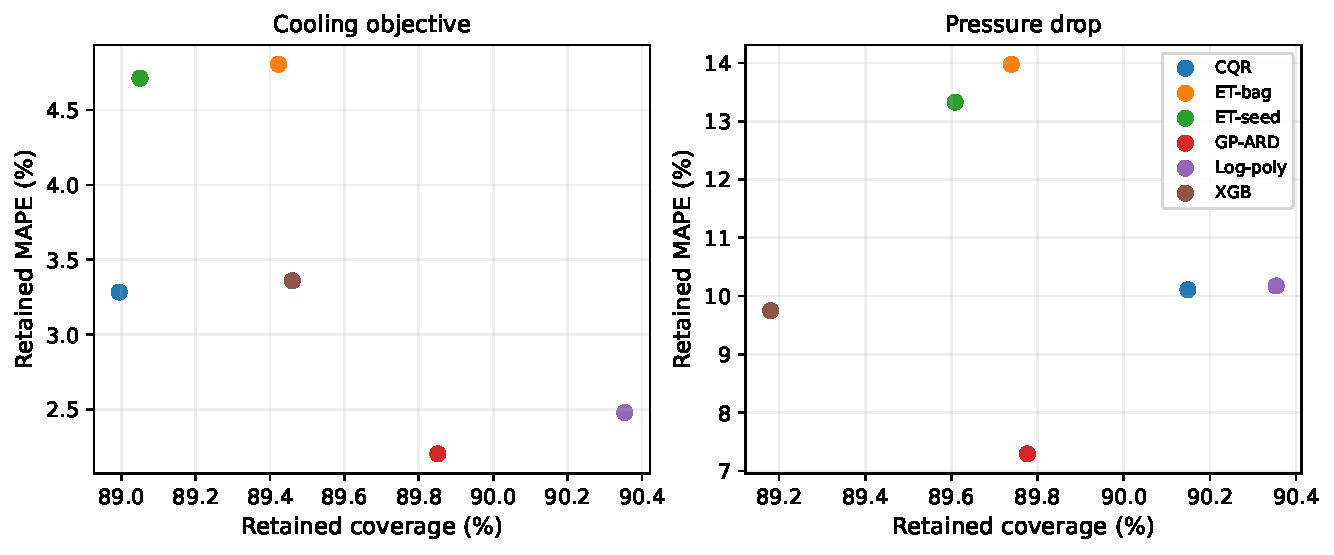
\includegraphics[width=\textwidth,height=.78\textheight,keepaspectratio]{../figures/coverage.pdf}\end{center}
\clearpage\section*{dataset}\noindent Response means in ten x0 bins across successful designs, averaged over other geometry coordinates; lines connect bin means, not additional CFD observations.\begin{center}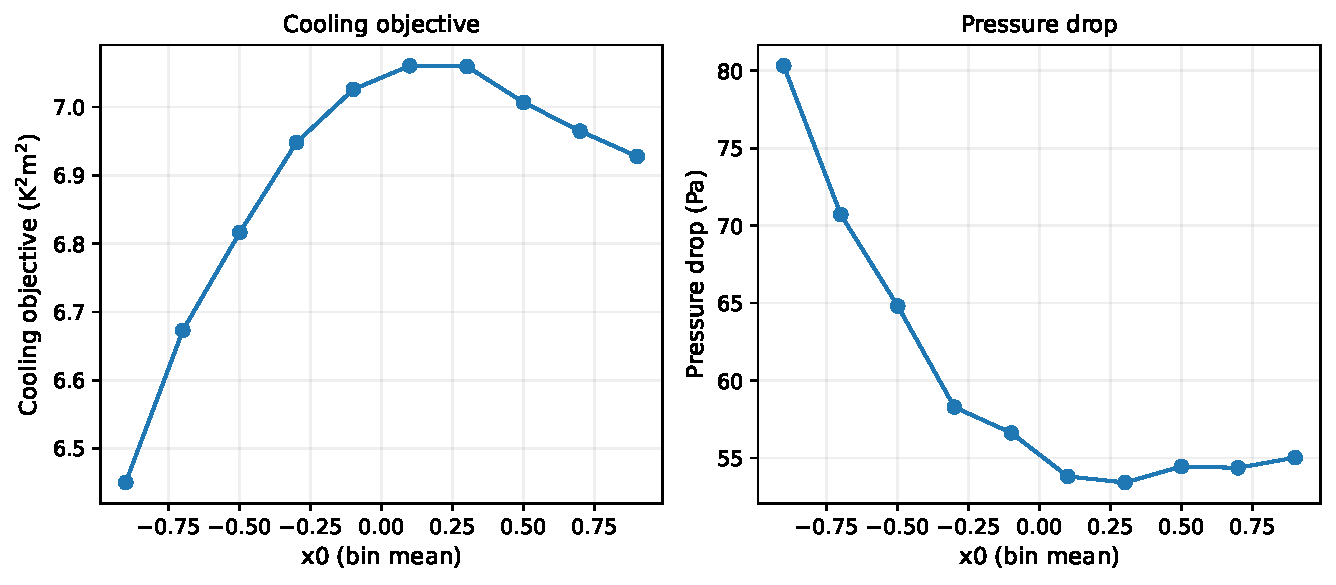
\includegraphics[width=\textwidth,height=.78\textheight,keepaspectratio]{../figures/dataset.pdf}\end{center}
\clearpage\section*{distance failure}\noindent Seed-42 high-x0 geometry-support test: response APE versus raw mean five-neighbor distance. Distances alone do not establish response error.\begin{center}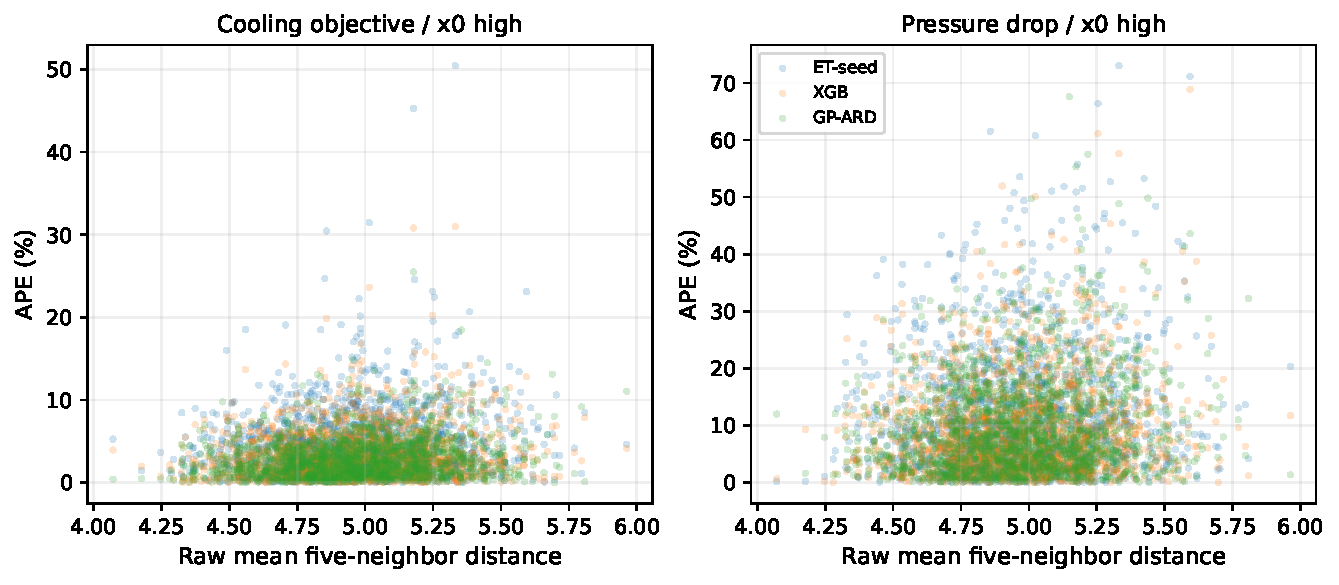
\includegraphics[width=\textwidth,height=.78\textheight,keepaspectratio]{../figures/distance_failure.pdf}\end{center}
\clearpage\section*{feature importance}\noindent Seed-42 ExtraTrees common-fit control on design-random data. Top ten impurity importances are descriptive, not causal physical effects.\begin{center}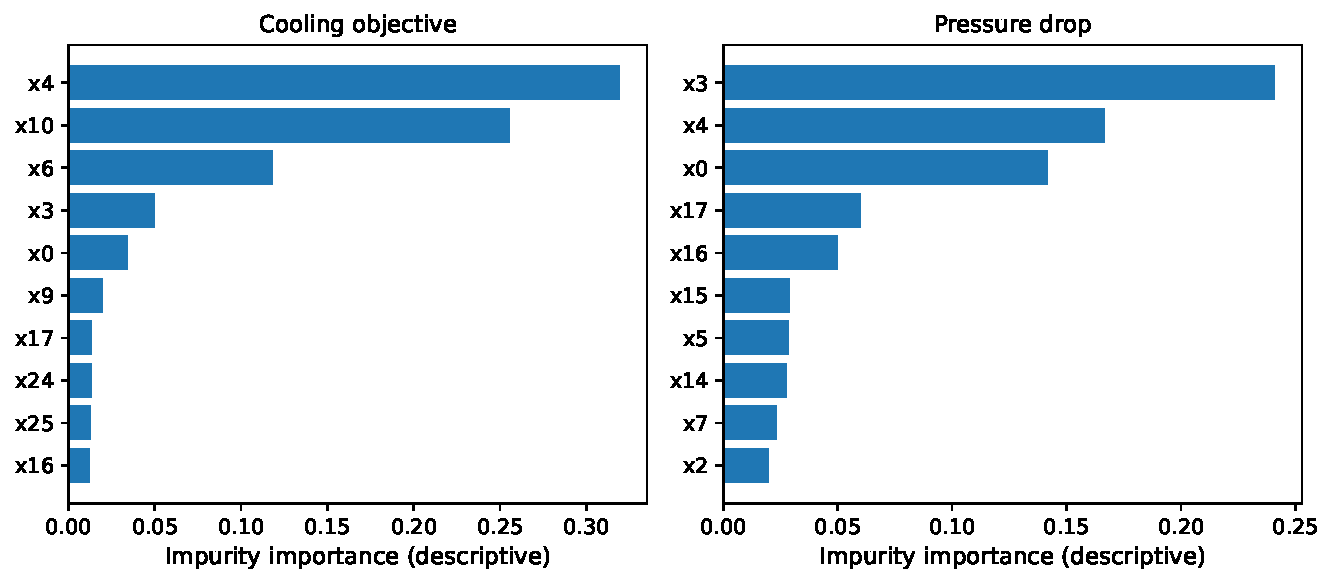
\includegraphics[width=\textwidth,height=.78\textheight,keepaspectratio]{../figures/feature_importance.pdf}\end{center}
\clearpage\section*{grouped parity}\noindent Seed-42 design-random test cases, same held-out designs across models. Dashed lines indicate exact agreement; axes show physical target units.\begin{center}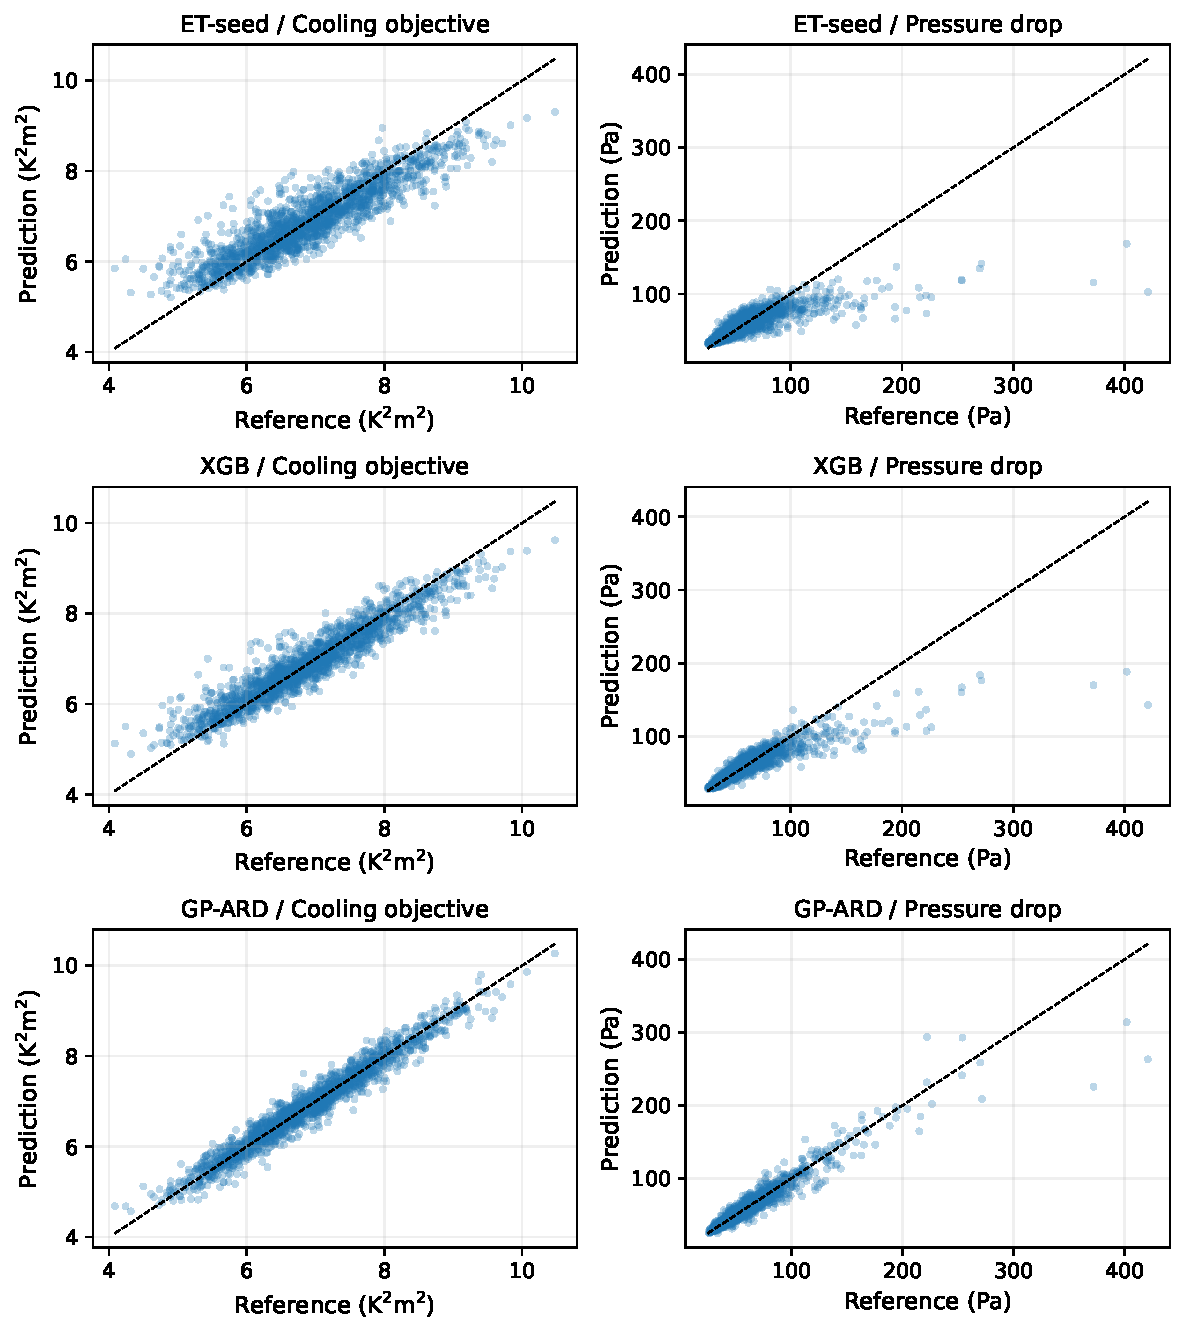
\includegraphics[width=\textwidth,height=.78\textheight,keepaspectratio]{../figures/grouped_parity.pdf}\end{center}
\clearpage\section*{map}\noindent Seed-42 design-random accepted fractions in x0/x6 quintile cells, averaged over actual test cases and all remaining geometry coordinates. Cell counts are supplied; this is not a full-grid physical validity map.\begin{center}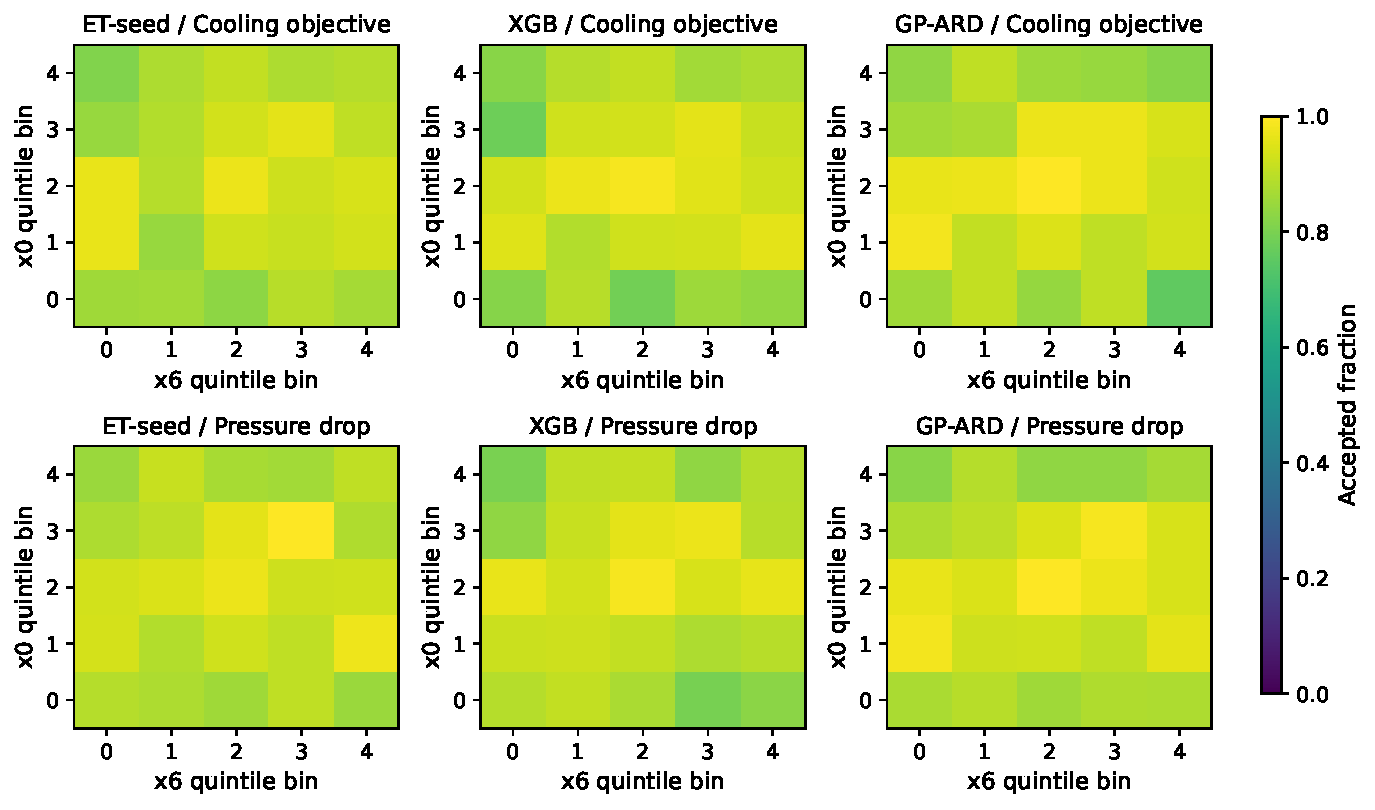
\includegraphics[width=\textwidth,height=.78\textheight,keepaspectratio]{../figures/map.pdf}\end{center}
\clearpage\section*{mixture}\noindent Common-model mixtures of supported and high-x0 test designs, averaged over three runs. False accepts use all test cases as the denominator; tolerances are illustrative.\begin{center}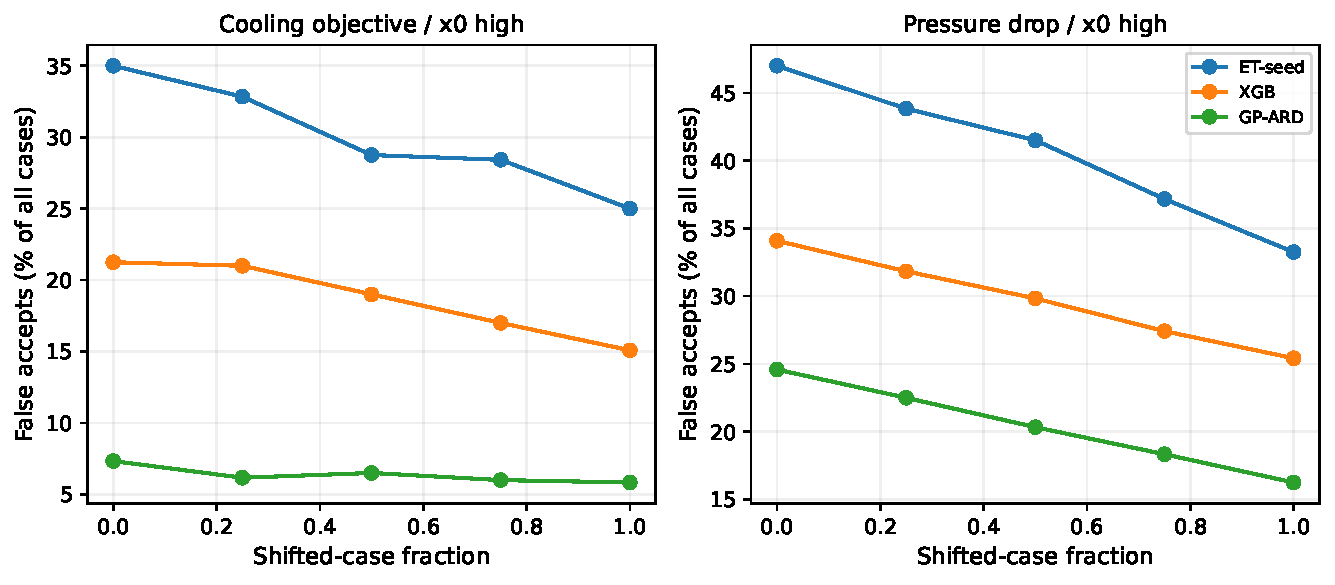
\includegraphics[width=\textwidth,height=.78\textheight,keepaspectratio]{../figures/mixture.pdf}\end{center}
\clearpage\section*{risk CoolingObjective K2m2}\noindent Cooling-objective seed-42 risk-coverage curves, separate folds, expected uniform ordering within score ties. These are retrospective rankings, not guaranteed deterministic threshold paths.\begin{center}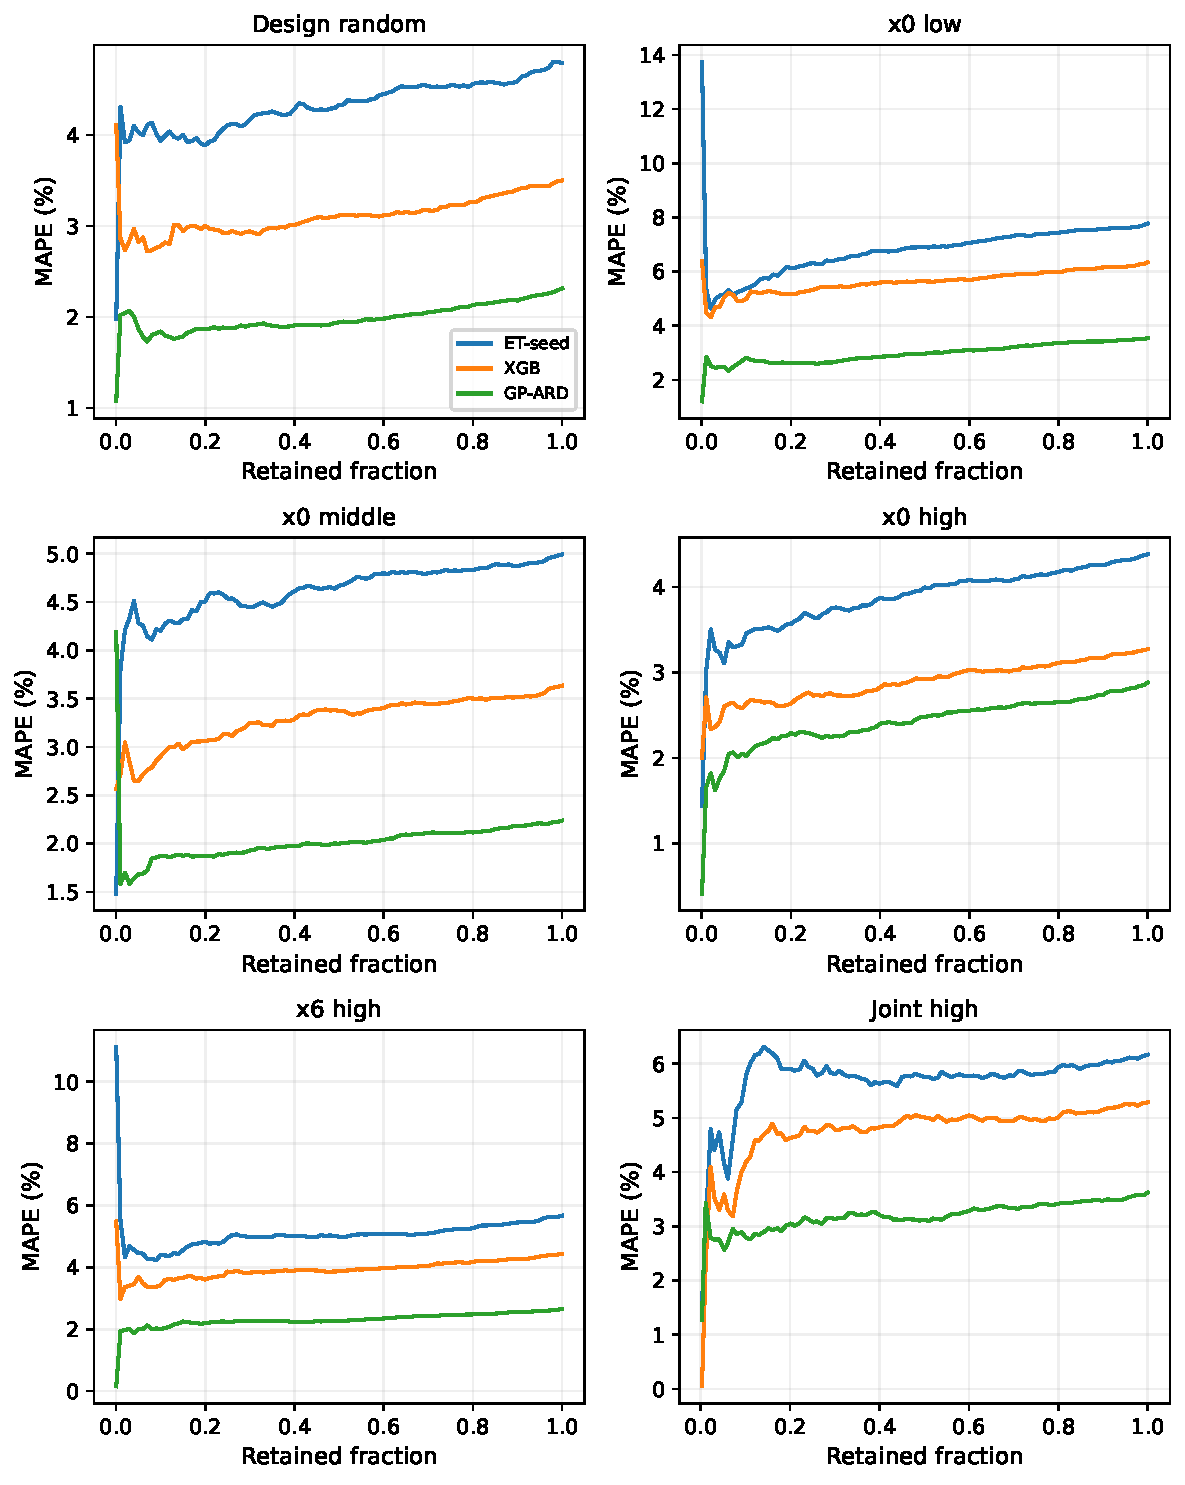
\includegraphics[width=\textwidth,height=.78\textheight,keepaspectratio]{../figures/risk_CoolingObjective_K2m2.pdf}\end{center}
\clearpage\section*{risk DelP Pa}\noindent Pressure-drop seed-42 risk-coverage curves under the same tie-aware, per-fold conventions; error is physical-unit MAPE in percent.\begin{center}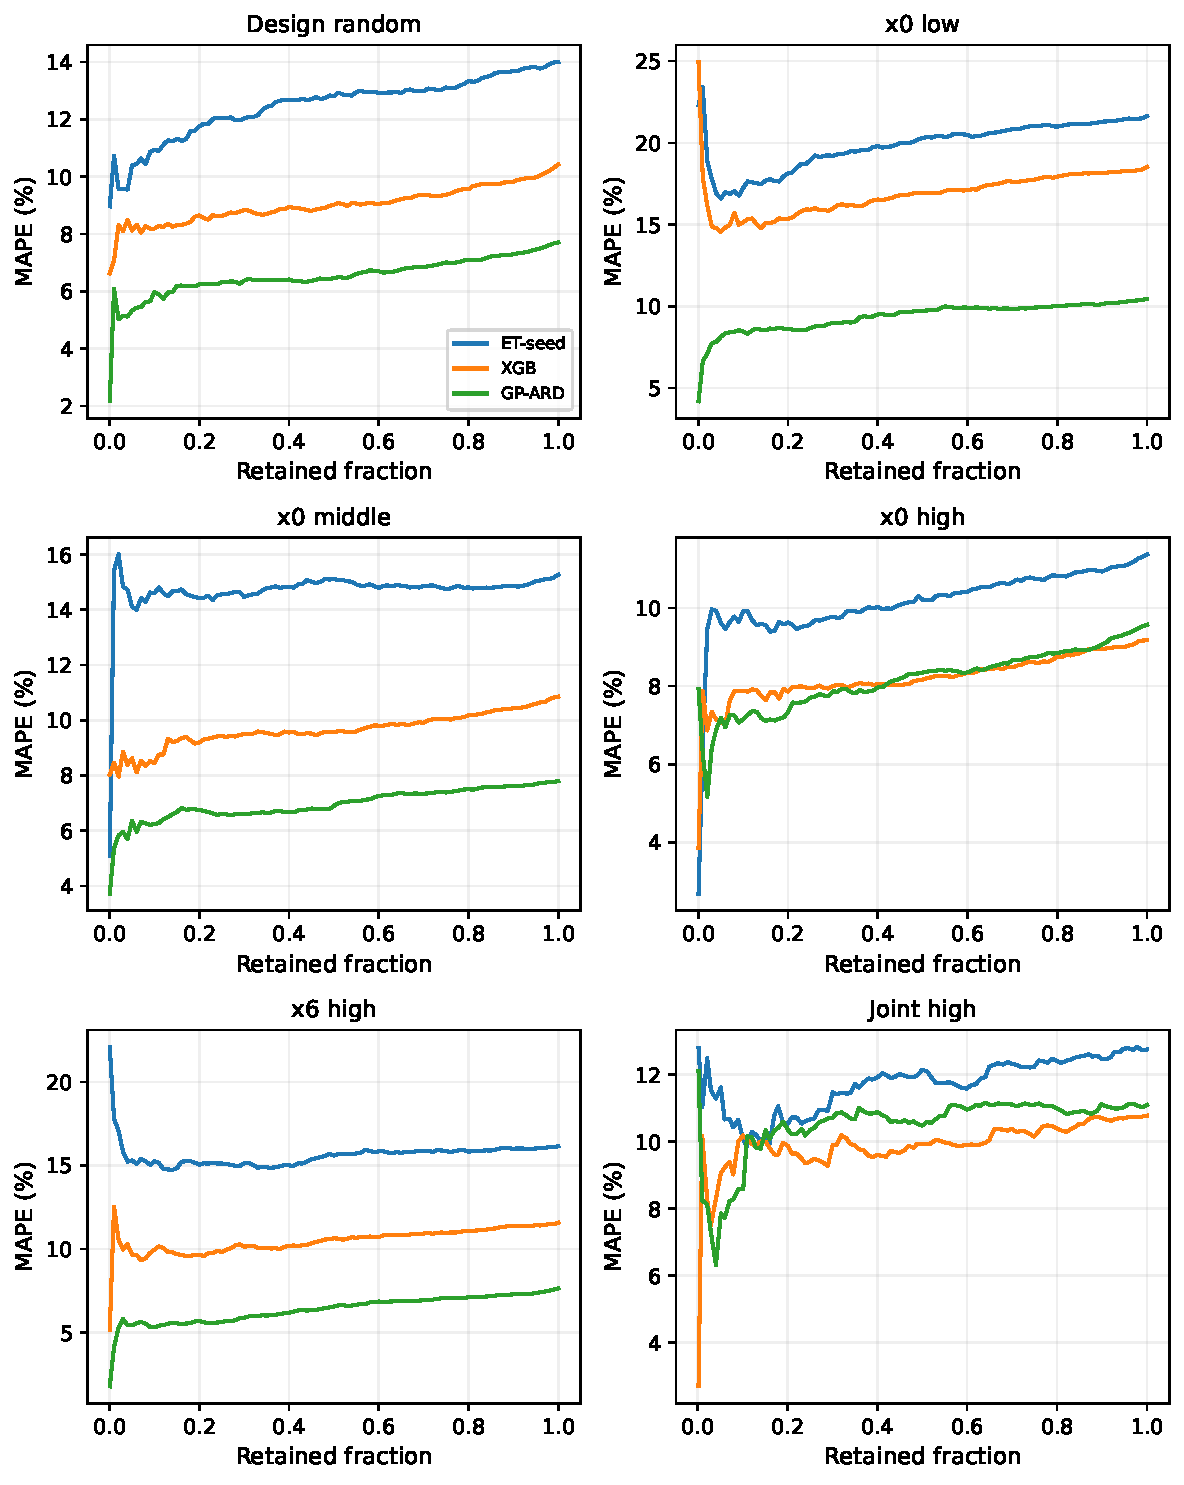
\includegraphics[width=\textwidth,height=.78\textheight,keepaspectratio]{../figures/risk_DelP_Pa.pdf}\end{center}
\clearpage\section*{scores}\noindent Seed-42 design-random XGB uncertainty, distance and fused score distributions. The dashed line is the independently calibrated max-score cutoff.\begin{center}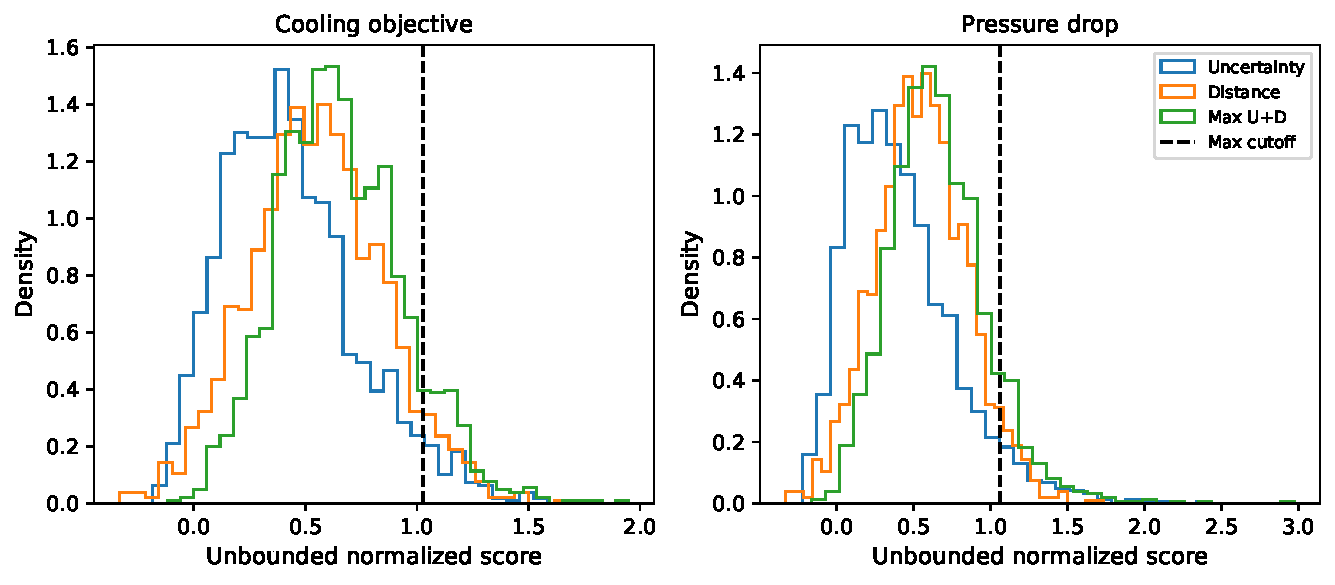
\includegraphics[width=\textwidth,height=.78\textheight,keepaspectratio]{../figures/scores.pdf}\end{center}
\end{document}